\chapter{Theoretical Framework}
\label{chapter:TF}

In this section, the core information needed for the comprehension of the desertion is presented. The RNA-seq analysis procedure is briefly explained alongside its application and the advantages of such technique over others. Moreover, the theoretical framework displays a concise state of the art of the algorithms employed in this RNA-seq analysis. Lastly, an outline of the possible molecular biomarkers in AD, PD and HD is introduced.

\section{RNA Sequencing} \label{rna-seq}

Forty years ago, Sanger sequencing methodology was considered innovative, although precise sizing of the termination products in polyacrylamide gels was very slow and arduous, and could not be applied to sequence large genomes. In 1990, capillary electrophoresis took advantage of the physically compact DNA separation and the fluorescent detection of termination products by the addition of four colored label termination reactions. Instead of employing a two-dimensional polyacrylamide gel, capillary electrophoresis miniaturized the page gel to a single dimension tube, a capillary. A computer-driven laser performed the detection of the fragments. Eventually, all these advancements generated a highly parallel automation sequencing which was not only cheaper and faster, but also facilitated the genome assembly. Thirty years ago, piecing together a 1.8 Mb genome sequence was viewed as a computational ordeal. Today, next-generation sequencing machines can produce 100 Mb in hours and analyzed with a personal computer \cite{Chapter1}.

Next-generation sequencing (NGS) technology makes reference to a new class of equipment that consists of rapid sample preparation and enhanced throughput at lower cost \cite{Lei2008}. Novel high-throughput RNA sequencing techniques have yielded new methods for mapping and quantifying transcriptomes; this technique is titled RNA-seq \cite{Wang}. Although each NGS platform accomplishes sequencing in a unique manner, some have a similar base methodology which includes library preparation, sequencing and imaging, and data analysis, as briefly presented in Fig. \ref{fig:RNA-seq-process}. Library preparation consists of building a repository of RNA, DNA or cDNA. These repositories are constructed by fragmenting the RNA or DNA sample and adding an adapter sequence (known sequence of synthetic oligonucleotides) to one or both ends of a fragment \cite{Grada}. Then, a short sequence, called read, is obtained from each fragment by employing high-throughput sequencing technology \cite{Wang}. After the raw reads have been obtained quality control checks must be made. Then, the transcript identification takes place, also called alignment; there are several algorithms which take care of this process, such as Bowtie, STAR, Cufflinks, kallisto, to name a few \cite{Conesa2016}.

\begin{figure}[h]
    \centerline{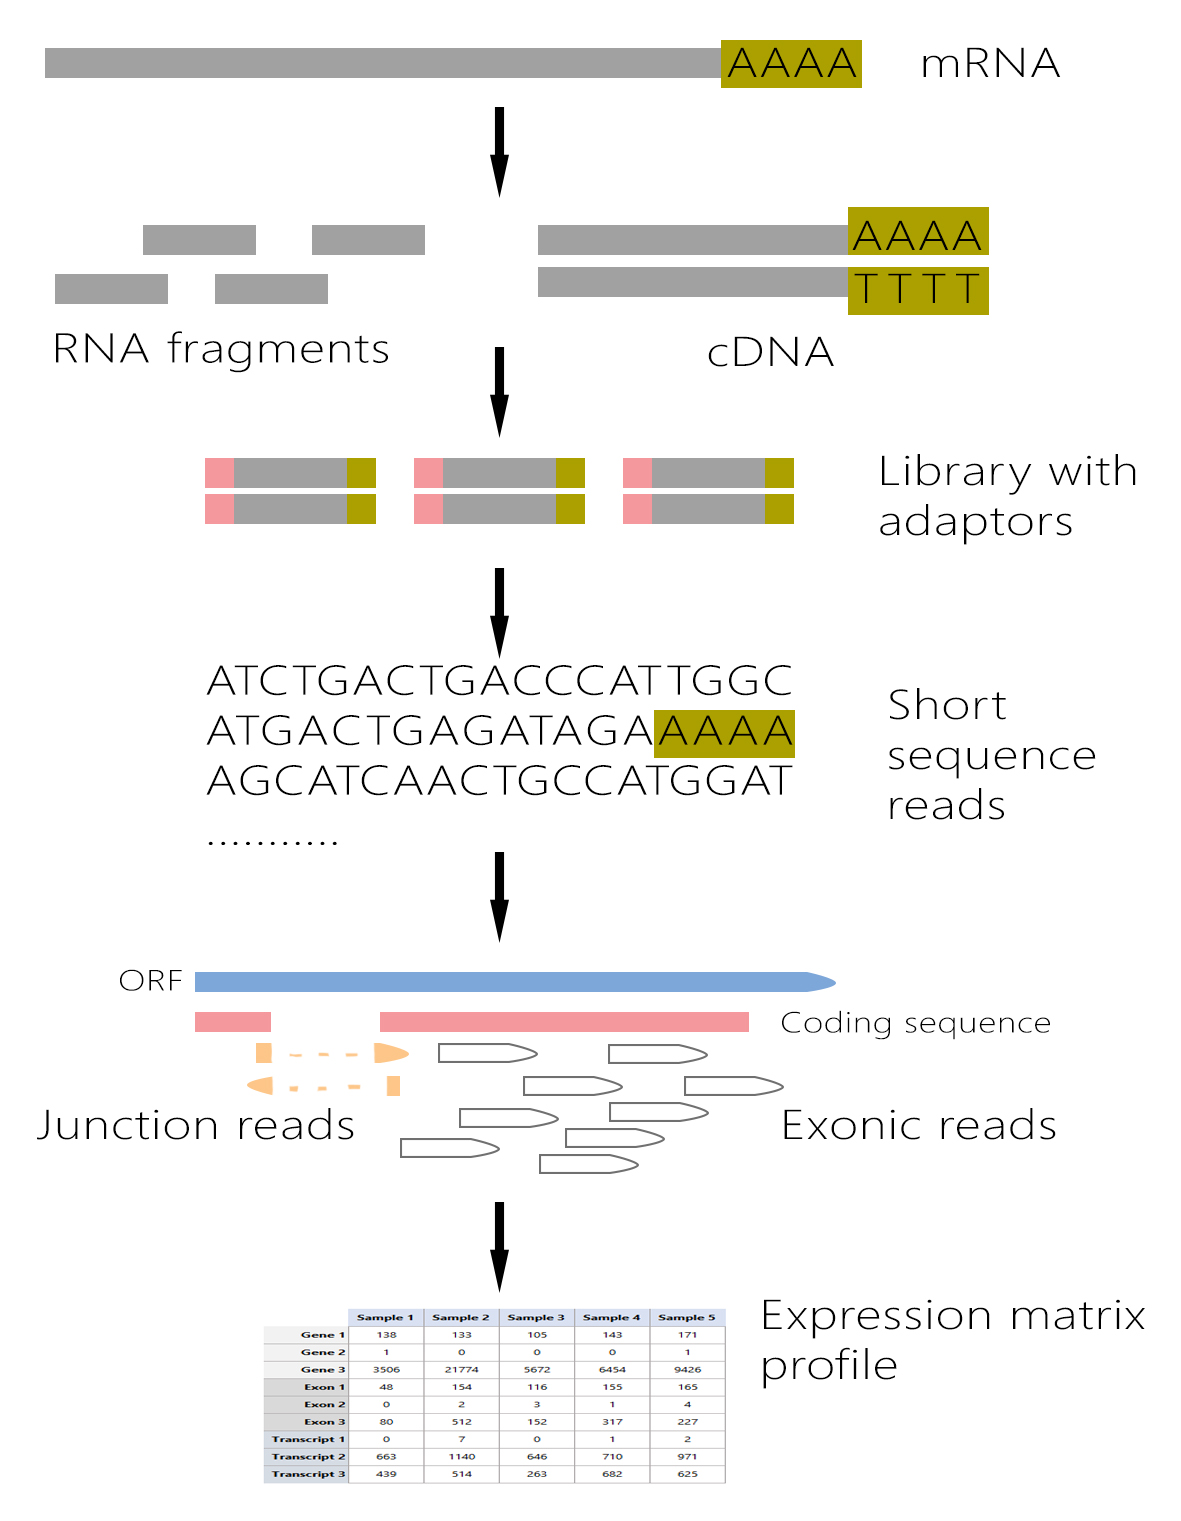
\includegraphics[width = 10cm]{Figures/RNA-seq-process-mat.jpg}}
\caption{Typical RNA-seq experiment (based on \cite{Wang}).}
\label{fig:RNA-seq-process}
\end{figure}

Transcript quantification is the most common application of RNA-seq which is based on the number of reads that map to each transcript sequence \cite{Conesa2016}. This measure can be discrete, i.e. number of reads, or continuous, such as reads per kilobase of exon model per million reads (RPKM), fragments per kilobase of exon model per million mapped reads (FPKM) and transcripts per million (TPM). On the other hand, DGE analysis requires the gene expression values in order to compare them between samples; the continuous measures are normalized as a way to discard highly variable or expressed features. The choice of normalization method can noticeably affect the outcome of the analysis. RNA-seq can perform other advanced analyses such as the identification of alternative splicing events, quantification at transcription, gene and exon level, isoform expression, analysis of small and other non-coding RNAs, single cell analysis, visualization and the integration with other omics \cite{Conesa2016}.

\section{RNA-seq Applications}

NGS has allowed rapid advancements in biological sciences by sequencing whole genomes and transcriptomes of a wide variety of organisms. By re-sequencing the human genome, novel genes and regulatory elements involved in pathological processes have been identified. Since mutations in gene-coding or control regions can give rise to unrecognizable clinical conditions, it is important to provide a fast, affordable and precise way to determine the genetic cause of a disease. Therefore, RNA-seq is capable of sequencing only the interesting protein-coding regions of the genome (exome), making the process more cost-effective considering that the exome comprises just 1\% of the whole genome \cite{Grada}. As mentioned above, RNA-seq is an open platform, a technology that does not depend on a genome reference, hence it enables the quantification of transcripts without predefining the targets of interest and generates enhanced detection of RNA splicing events. Also, RNA-seq can characterize undefined transcripts of other RNA species such as microRNAs (miRNA), PIWI-interacting RNAs, tRNAs, RNA precursors, among other intra- and extracellular species; the aforesaid sets many opportunities for RNA-seq in the clinical test environment \cite{Byron}. In Table \ref{table:RNA-mol}, examples of RNA molecules applications are presented.

\begin{table}[ht]
\centering
\caption{Examples of RNA molecules and their applications \cite{Byron}.}
\label{table:RNA-mol}
\begin{tabular}{ll}
\hline
\multicolumn{1}{c}{\textbf{RNA molecule}} & \multicolumn{1}{c}{\textbf{Application}}      \\ \hline
Viral RNA                                 & Viral detection and characterization          \\
mRNA                                      & Diagnosis and prognosis                       \\
miRNA                                     & Diagnosis                                     \\
\multirow{3}{*}{Fusion transcript}        & Diagnosis                                     \\
                                          & Monitoring molecular response to drug therapy \\
                                          & Fusion detection                              \\ \hline
\end{tabular}
\end{table}

Moreover, genetic variants like single-nucleotide polymorphisms (SNPs) within intronic or intergenic regions, are now associated to complex diseases and traits suggesting that these variants are likely to have causal effects by affecting gene expression rather than protein function; sections of chromosome which have affected gene expressions are referred as expression quantitative trait loci (eQTL). eQTL analysis provides a way to research complex traits and the pathogenesis of some diseases, and RNA-seq may correspond to the working rule for a high-resolution eQTL analysis \cite{Costa}. Furthermore, RNA-seq analysis is capable of giving functional insights into pre-mRNA processing and isoform expressions; distinct isoforms formed from alternative spliced genes are relevant in the development and differentiation of a cell and its diseases \cite{Katz}. Lastly, GSEA can be applied with RNA-seq providing the identification of possible altered pathways in some condition, like diseases or during drug treatment \cite{Subramanian}. RNA-seq is at the bound of possibility in genomic technology.

\section{Advantages Over Other Sequencing Methods}

For the past decades, DNA microarrays have been a powerful approach to achieve examination of biological systems at a genomic scale. Microarrays applications included transcriptome analysis, profiling of protein-DNA interactions, and characterization of small-scale and large-scale genetic variation. This technique has influenced the scientific community to collect and analyze large-scale datasets. Microarrays are a hybridization-based technology, which possesses some limitations: the sequences analyzed must be known; cross-hybridization occurs when highly related sequences are being examined; the analog signals makes it difficult to detect and quantify low and very high abundance species; and discrepant results between laboratories and platforms \cite{Shendure}. Nonetheless, hybridization-based methods are high-throughput and relatively inexpensive. Tag-based technology is another approach for genome and transcriptome analysis (SAGE, CAGE and massively parallel signature sequencing (MPSS)) and was developed to overcome some of the limitations of microarrays. However, these methods are based on Sanger sequencing which is expensive, and a considerable fraction of short tags cannot be exclusively mapped to the reference genome \cite{Wang}. RNA-seq has clear advantages over existing technologies and is expected to transform the manner in which cells transcriptome is analyzed. As mentioned throughout the text, RNA-seq possesses numerous benefits which are summarized in Table \ref{table:advantages} presented below (relative to other sequencing technologies, such as microarrays).

\begin{table}[ht]
\centering
\caption{Technological benefits of RNA-seq, relative to other sequencing technologies \cite{Wang}.}
\label{table:advantages}
\begin{tabular}{ll}
\hline
\multicolumn{1}{c}{\textbf{Technology specification}}                                                                                                                             \\ \hline
Throughput                                                                                           & High                                                                                                           \\
Resolution                                                                                           & Single base                                                                                                    \\
Reliance on genomic sequence                                                                         & In some cases                                                                                                  \\
Background noise                                                                                     & Very low                                                                                                       \\
\begin{tabular}[c]{@{}l@{}}Simultaneously map transcribed regions\\ and gene expression\end{tabular} & Yes                                                                                                            \\
\begin{tabular}[c]{@{}l@{}}Dynamic range to quantify gene\\ expression level\end{tabular}            & \textgreater 8,000-fold                                                                                        \\
Ability to distinguish allelic isoforms                                                              & Yes                                                                                                            \\
Ability to distinguish allelic expression                                                            & Yes                                                                                                            \\
Required amount of RNA                                                                               & Low                                                                                                            \\
Cost of mapping transcriptomes of large genomes                                                      & \begin{tabular}[c]{@{}l@{}}Relatively low\\ (\textless \$1,000 USD \cite{Grada})\end{tabular} \\ \hline
\end{tabular}
\end{table}

\section{Tools and Algorithms}

The algorithms and tools for the first steps of RNA-seq analysis, meaning library preparation, sequencing and imaging, will not be mentioned in this desertion since the solution employs processed RNA-seq expression data. Hence, the explained tools are those contained in the phase of data analysis. On the other hand, the whole pipeline was performed in R version 3.6.2 \cite{R} and RStudio \cite{RStudio}.

\subsection{Download and Preprocessing}

As described in Fig. \ref{fig:solution-overview}, the first step is to download the processed RNA-seq and clinical data from GEO. For this, the R package, \textit{GEOquery} \cite{GEOquery}, was leveraged. \textit{GEOquery} is the bridge between GEO and BioConductor \cite{bioConductor}. The latter is an open-source software project for the analysis of genomic data which contains many of the state-of-the-art tools and methods. The former is a public repository that was developed by the National Center for Bioinformatics (NCBI) at the National Institutes of Health (NIH) and contains around 140,000 gene expression experiments. Therefore, this tool eliminates many parsing and formatting problems, and facilitates the analyses and meta-analyses of genomic data \cite{GEOquery}. \textit{GEOquery} is part of BioConductor.

After quering the required databases, a common used tool is \textit{biomaRt} \cite{biomart}, another BioConductor package. \textit{biomaRt} is an application programming interface to BioMart web services developed by the Ontario Institute for Cancer Research and the European Bioinformatics Institute. This tool is also a bridge which connects BioMart data resources (e.g. Ensembl) and BioConductor project, creating an environment for data mining. It allows the retrieval of large amounts of biological data (such as gene symbol, chromosomal coordinates, and OMIM annotation) in an uniform and easy way, and can annotate a varied gene or gene product identifiers \cite{biomart}.

Normalization is an important step in the preprocessing of many data analyses. In this study, \textit{preprocessCore} \cite{preprocessCore} package, contained in BioConductor as well, was leveraged for this purpose. This package is a library of core preprocessing methods which includes quantile normalization, background correction, among others. Subsequently, another significant step must be done: removing batch effect. Batch effect occurs when samples are processed and measured in different batches, different days, different groups or by different people, and it represents the systematic technical difference unrelated to any biological variation \cite{sva}. Moreover, it is the best-known source of latent variation in genomic experiments \cite{leek}. In order to solve this problem, the R package \textit{sva} \cite{sva} was used. \textit{sva} includes different methods which identify and directly remove known batch effects and other unknown sources of variation by estimating surrogate variables. Using these methods have shown to reduce dependence, stabilize error rates and improve reproducibility \cite{leek}. \verb|ComBat| is the batch correction function of \textit{sva}; it uses a parametric or non-parametric empirical Bayes framework in order to adjust the high-dimensional data and output corrected measurements without batch effects \cite{sva}.

\subsection{Covariates and molecular subtypes}

In order to identify relevant covariates in the data, \textit{limma} was used. This package is explained in the following subsection. Following, the core samples had to be selected from the data, meaning appointing the samples most representative of the group of each database; those that have higher similarity to their own condition than to the other. To perform this step, NMF was leveraged. NMF is a widely used tool for the analysis of high dimensional data since it extracts meaningful features from a set of non-negative vectors. It is a linear dimensionality reduction method which was introduced in 1994 by Paatero and Tapper \cite{paatero} and gain popularity after Lee and Seung \cite{lee} presented the method as an unsupervised learning paradigm in 1999. The objective of NMF is to decompose a data matrix $X$ into $WH$ ($X \approx WH$), where $W \geq 0$ and $H \geq 0$, which means that $W$ and $H$ are component-wise non-negative matrices \cite{gillis}. Few years back, NMF was primarily used in image and natural language processing. However, recently, it has been successfully applied in applications of computational biology: functional characterization of genes, cross-species analysis, class comparison, and molecular pattern discovery. In the context of genomic data, the matrix $X$ consists of observations on $p$ genes from $n$ samples, resulting in a gene expression matrix of $p \times n$. Each column of matrix $W$ describes a metagene, and each column of matrix $H$ characterizes the metagene expression pattern of the matching sample. Moreover, matrix $W$ has a size of $p \times k$, and matrix $H$ has a size of $k \times n$ where $k$ is the rank of factorization and defines the number of latent factors in the decomposition process \cite{nmf}. In this study, NMF was leveraged for the selection of core samples and also for molecular subtype analysis (mentioned before as molecular pattern discovery); for the former, $k$ was set to two (control and case grouping) and for the latter, this value has set to a range of two to five clusters.

\subsection{Cell type proportions} \label{cellprop}

Another additional analysis is the characterization of cell composition of complex tissues in bulk RNA-seq data. The Cell-type Identification By Estimating Relative Subsets Of RNA Transcripts (CIBERSORTx) \cite{Newman} algorithm, from the Alizadeh Laboratory and Newman Laboratory of Stanford University, is an analytical tool which estimates the fractions of multiple cell types in gene expression profiles; it resembles an \textit{in silico} flow cytometry. CIBERSORTx was engineered in a web framework based on R and PHP in order to reduce dependencies on specific hardware and software. This algorithm requires as input a gene expression data of a bulk mixture of different cell types, and a signature matrix file which acts as reference for each cell type of interest. The signature matrix can be obtained from curated datasets, or from custom signature gene files by supplying the reference gene expression profiles of pure cell populations \cite{Steen}. Moreover, the noise of the datasets are removed with a linear support vector regression, a machine learning technique \cite{Newman}. Afterwards, the tool generates the fractional representations of each cell type contained in the mixture and returns a heatmap, stacked barplot and the quantitative values of these representations. Recently, the authors enhanced the algorithm by giving the option to use signature matrices derived from single-cell RNA-seq data.

A similar approach can be made by Brain Cell Type Specific Gene Expression Analysis (\textit{BRETIGEA}) \cite{bretigea}. This R package is akin to CIBERSORTx, since it also performs an analysis of relative cell type percentages in bulk gene expression data. \textit{BRETIGEA} is specific to brain cell types, as its name describes, and it contains validated set of brain cells marker genes originated from various experiments, as defined in \cite{mckenzie}. Moreover, the marker genes are accessible for astrocytes, endothelial cells, microglia, neurons, oligodendrocytes, and oligodendrocyte precursors (Opc) from human and mouse. Nonetheless, the functions can be applied to marker genes from any other tissue obtained by the user. Additionally, the number of marker genes used in the analysis can be modified in order to adjust to the user's preference and the given dataset \cite{bretigea}.

\subsection{Differential gene expression analysis} \label{limma-method}

The main objective of DGE analysis is to statistically test if a given quantitative expression of a gene changes between two or more conditions (experimental groups) or are associated with specific predictors or responses. The basic tasks of the analysis are (i) to estimate the magnitude of the differential expression between the conditions, i.e. fold change of expression, and (ii) estimate the significance of the difference of this change and correct it for multiple testing, i.e. p-value and q-value \cite{dundar}.

A common method for DGE analysis is \textit{limma} \cite{Ritchie}, a BioConductor software package for analyzing data from gene expression experiments. The package contains tools for reading, normalizing and exploring such data. Also, \textit{limma} is capable of performing differential splicing analysis. \textit{limma} operates on a matrix of expression values with columns as samples and rows as expression values. This tool uses linear models to explore entire experiments as an integrated whole rather than making comparisons between pairs of treatments; this creates an effect of sharing information between samples and allows to model correlations that may exist between those samples (empirical Bayes). Moreover, linear models are flexible and permit to test interactions effects or more complex comparisons between groups. In differential expression testing, gene-wise variances are squeezed towards the common variance; this reduces the number of false positives for genes with small variances and enhances the effectiveness to detect differential expression for genes with bigger variances. Lastly, the memory requirements are linear in the number of genes and the number of samples \cite{Ritchie}.

\subsection{Functional analysis}

In the last steps of the standard RNA-seq analysis, the interpretation of the results can be made by functional profiling methods, i.e. the characterization of the molecular functions or pathways where differentially expressed genes (DEGs) are implicated. One such method is GSEA which is based on ranking the transcriptome according to the differential expression \cite{Conesa2016}. GSEA focuses on groups of genes that share biological functions, chromosomal location, or regulation; these groups are called gene sets. The main objective of the algorithm is to determine if the members of a gene set tend to occur toward the top or bottom of an ordered list according to their differential expression between the classes. This tool contains three key elements: enrichment score (ES), the statistical significance of the enrichment score (SSES), and the normalized enrichment score (NES) to calculate the false discovery rate (FDR). The first element reflects the degree to which a gene set is over represented at the extremes of the list. ES is the maximum deviation from zero encountered in a random walk down the list; the score increases when a gene of the set is encountered and decreases when genes are not in the set. The SSES is estimated by using an empirical phenotype-based permutation test; the phenotypes labels are permutated, and the ES is recomputed generating a null distribution for the ES. The empirical nominal p-value is calculated relative to this null distribution. Lastly, the ES is normalized by considering the size of each gene set; then the FDR is calculated by controlling the proportion of false positives corresponding to each NES (computed by comparing the tails of the observed and null distributions for the NES). At the end, GSEA returns the groups which can correspond to the same biological processes and which represent distinct processes \cite{Subramanian}.

To accomplish the functional profiling mentioned above, two R packages were utilized: \textit{MSigDBr} \cite{msigdbr} and \textit{clusterProfiler} \cite{clusterprofiler}. The first package provides the Molecular Signatures Database (MSigDB) gene sets, biological ontologies, used for GSEA in a standard data frame with key-value pairs and one gene per row. It includes gene symbols and NCBI/ Entrez gene IDs for human, mouse, pig, rat, yeast, fly and zebrafish. An advantage of this package is that it is installed and loaded without the need of additional external files \cite{msigdbr}. On the other hand, \textit{clusterProfiler} automates the process of GSEA and term classification by combining the analysis and visualization into one workflow. It was designed to compare biological themes among gene clusters with the statistical analysis of Gene Ontology (GO) \cite{GO} and Kyoto Encyclopedia of Genes and Genomes (KEGG) \cite{KEGG} ontologies. Moreover, \textit{clusterProfiler} can also be applied to clusters from protein-protein interactions and miRNA target genes \cite{yu}. It is important to mention that this package implements the GSEA algorithm proposed by Sergushichev, named Fast Gene Set Enrichment Analysis (FGSEA), which permits to make more permutations and get finer p-values \cite{fgsea}. Additionally, this package is a part of BioConductor project.

Over representation analysis (ORA) is another common approach for functional analysis \cite{ora}. This approach determines if biological functions or processes are over represented in a list of DEGs; the over representation can also be called enrichment. The p-values are calculated with a hypergeometric test adjusted for multiple comparison. ORA finds genes with a large difference in expression, but it does not detect situations where this difference is small. These situations are seen in a coordinated way by the set of related genes. Nonetheless, this limitation is addressed by GSEA approach \cite{clusterprofiler}. Both methods, ORA and GSEA, can be performed by \textit{clusterProfiler}. As said before, \textit{clusterProfiler} can analyze and visualize the comparisons in the same module by leveraging \textit{enrichplot} \cite{enrichplot}, a visualization package based on \textit{ggplot2} \cite{ggplot2} which implements several visualization methods to aid in the interpretation of the ORA and GSEA results \cite{clusterprofiler}.

\subsection{Drug repurposing}

Some other analyses can be performed over RNA-seq data, such as drug repurposing, by generating disease gene expression signatures through a comparison of gene expression of control and disease sample; each signature contains key genes, called landmark genes. The major result is the reverse gene expression score (RGES), which indicates if a drug can reverse the disease gene expression (low negative value) or not. Moreover, the summarized RGES is a score that represents the overall reversal potency of a compound to a particular condition, which successfully correlates with drug efficacy. Correspondingly, RGES can be applied to unravel some mechanisms of action of drug candidates by studying the genes reversed by the drug \cite{Chen}.

In this research, \textit{PharmacoGx} \cite{pharmacogx} was used for this purpose. \textit{PharmacoGx} is an R package which allows to download and examine large pharmacogenomic datasets; these are thoroughly curated datasets in order to ensure maximum consistency. This package contains parallelized functions to evaluate the reproducibility of molecular and pharmacological data, and identify the molecular features which are uniformly related with drug effects. \textit{PharmacoGx} employs the Connectivity Map (CMAP) project \cite{lamb} as "drug perturbation datasets", since the project characterized the transcriptional changes caused by an extensive set of medications. Using the \verb|connectivityScore| function the disease signatures can be compared against drug signatures (from the drug perturbation datasets), and it outputs a list of possible treatments \cite{pharmacogx}.

\subsection{GWAS variations} \label{gwas}

GWAS provide the opportunity to explore the impact of common variants on complex diseases. Therefore, to compare these variants with the resulted DEGs, first, the GWAS database was downloaded from GWAS Catalog \cite{gwascat}. The GWAS Catalog was founded by the National Human Genome Research Institute (NHGRI) at the NIH in 2008, and is now a collaborative project with the EMBL-EBI. The Catalog gives a consistent, searchable and freely available database of SNP-trait relations. All the studies contained in the GWAS Catalog are identified and evaluated by the curators of the team; they extract the reported trait, SNP-trait relation, and metadata. Since 2020, GWAS Catalog is also accepting submissions of unpublished data. As of February 2021, the GWAS Catalog includes 4,892 publications and 248,356 associations. Moreover, the data is mapped to Genome Assembly GRCh38.p13 and dbSNP Build 153 \cite{gwascat}.

After selecting the variants of interest from the GWAS Catalog database, the Single Nucleotide Polymorphism Annotator (SNiPA) \cite{snipa} online tool was used to query for variants that are in linkage disequilibrium (LD) within a 500 kb window. SNiPA, a tool for annotating and browsing genetic variants, is a project developed by the Institute of Computational Biology at the Helmholtz Zentrum München and the Bioinformatics Core Facility at the Weil Cornell Medical College in Qatar. This tool combines the LD data of 1000 Genomes Project with gene annotations, trait relations, and eQTLs \cite{snipa}.

Subsequently, the selected variants of GWAS Catalog and those obtained with SNiPA were input to Polymorphism Phenotyping v2 (PolyPhen-2) \cite{polyphen} web server in order to predict a possible impact on the structure and function of a protein. PolyPhen-2 is a tool for the annotation of non-synonymous SNPs. The latter concept refers to the SPNs which are located in coding regions and result in protein variations of amino acids causing an effect on the function or structure of such protein. Additionally, the annotations of PolyPhen-2 comprises of around 150 million mis-sense codon changes in the exons of 43,043 UCSC gene human transcripts (hg19/ GRCh37). Lastly, this tool predicts the impacts based on a probabilistic classifier for all the resulting amino acid residue substitutions in UniProtKB proteins \cite{polyphen}.

Finally, the variants which were not mapped to any protein variation were queried in RegulomeDB \cite{regulomedb}. RegulomeDB is a database developed by Stanford University and the University of Michigan. This database is used to detect DNA regulatory elements and features in non-coding regions of the human genome. RegulomeDB includes regions of DNase hypersensitivity, transcription factor binding sites, and promoter regions which play a role in regulation transcription. The data is sourced from public datasets from GEO, the ENCODE project \cite{encode}, and other published literature, and includes manually curated regions involved in regulation (protein binding sites and motifs), ChIP-seq data for regulatory factors, chromatin state information, and eQTL data \cite{regulomedb}. With this information, RegulomeDB scores the inquired variants in order to separate the interesting variants from the pool. The data of RegulomeDB queries to dbSNP build 153 and maps to the human genome sequence hg19.

\section{Biomarkers for ND}

AD, PD and HD are neurodegenerative conditions that result from the gradual and progressive loss of neurons \cite{Costa}. These three diseases are diverse in their pathology and cause memory and cognitive impairments, from speaking to breathing. Deep comprehension of NDs' origins and mechanisms is must needed in order to generate effective treatments. In the past years, some insights of NDs mechanisms have been acquired through animal models and induced-pluripotent stem cells from different human cells due to the inaccessibility of the human brain. Furthermore, evidence proposes that NDs are not only induced by dying neural cells; in 2011, Twine et al. presented a thorough analysis of post-mortem brain samples of AD patients using RNA-seq technology. The authors observed that aberrations in the control of gene expression contributed to the initiation of AD, particularly alternative splicing \cite{Twine}. Nonetheless, non-neuronal cells play major roles in the disease development. In the case of PD, studies have shown that the disruption of calcium homeostasis can trigger the pathology. In order to predict a ND before the symptoms appear, microsatellites must be identified, and RNA-seq have this potential \cite{Gitler}. NDs are a significant problem in this era due to the aging of the overall population. Today 10 million people worldwide are living with PD; it is estimated that 50 million people are diagnosed with AD; and 205,000 people are affected by HD \cite{Marras, WAR, PringsheimHD}.

Addressing the NDs is compelling. The population with AD and PD is estimated to rise due to the aging of the population combined with the increase in life expectancy. The population affected by AD is expected to reach 131 million of individuals by 2050; just today the estimated worldwide cost of dementia is of trillions of US dollars \cite{WAR}. Some studies project that the number of patients with PD will double over the next 30 years, climbing to more than 12 million patients worldwide in 2050. Nonetheless, a greater increase can be expected if the population continues to age, medical management keeps improving and the environmental risk factors remain stable or rise \cite{Rocca}. Together, direct and indirect cost of PD is estimated to be nearly \$52 billion US dollars per year only in the United States \cite{Marras}. On the other hand, HD prevalence has increased from decades ago until now: 15-20\% per decade in Australia from 1954 to 1996; in North America from 1950 to 2012; and Western Europe from 1930 to 2007 \cite{Rawlins}.

GWAS have contributed to the knowledge of how common genetic variability reports risk development of complex diseases. Currently, advances in technology have allowed the analysis of very large numbers of markers throughout the genome, which is the approach used by GWAS. Nonetheless, complete biological pathways are still not complete. For example, for PD GWAS identified that genes involved in Mendelian form also modulate risk for the more common and sporadic form of this disease. Likewise, it has been reported by GWAS that apolipoprotein E is the most significant risk factor for AD \cite{Bras}. Following, novel identification of differential expression genes using RNA-seq data for AD, PD and HD is presented.

A recent study using frozen brain tissue from three regions, identified a total of 2,122 DEGs between AD samples and controls, from which 2,075 are protein coding genes and 47 are long non-coding RNAs (lncRNA). The mentioned genes are related to regulation of important neurological functions, such as synaptic long-term potentiation, neuronal signaling, axonal guidance signaling and mitochondrial dysfunction. Also, several genes are involved in pathways regulated by the miR-132/212 cluster; this cluster is a potential family related to AD pathogenesis which is normally downregulated in disease conditions. Furthermore, a positive upstream regulator of this cluster, BDNF, was found to be downregulated. Additionally, the four differential expressed miRNAs were all downregulated and were detected in 6 pathways: MAPK and neurotrophin signaling, axon guidance, long-term potentiation, glutamatergic and cholinergic synapses. On the other hand, the authors indicated that the original cellular population was preserved, and differential expression of cell-type specific genes was not affected. Finally, NR4A2 gene encodes an orphan nuclear receptor, which plays important roles in neural processes; the study suggested such protein may be involved in AD pathology because it was localized prominently in brain regions with A$\beta$ plaque accumulation \cite{Annese}.

From the study \cite{Annese}, 19 protein-coding differential expressed genes were detected between PD samples and controls. Additionally, miRNAs, which are deregulated, are enriched in some neuronal and inflammatory pathways; these miRNAs are entailed in general responses to brain injury. Another study concluded that differential gene expressions of PD samples were altered in NAD biosynthesis and recovery \cite{Bennett}. On the other hand, through the application of GWAS, 49 loci have been highlighted to associate with sporadic PD predisposition, from which many prioritized genes, like PARL gene, have been shown to impact mitochondria; its dysfunction has been widely implicated in PD \cite{Hook}. Also, gene SNCA (encodes for $\alpha$-synuclein) and MAPT (encodes for microtubule-associated protein tau) are known risk loci \cite{Bras}; the latter was found to have a variation in the exon 3 splicing which explains the genetic association to the disease. A large-scale transcriptome association study approach concluded with the identification of 66 genes whose expression or splicing are meaningfully related with PD risk. From these genes, some genetic risk factors influence innate-immune mechanisms \cite{Li}.

Last, it is widely known that HD is caused by a mutated CAG repeat in the huntingtin gene which encodes an expanded polyglutamine tract, the huntingtin protein. Huntingtin is involved in vesicle transport and transcriptional regulation. This mutant protein is modified into several smaller fragments; the origin of the small fragments which are found in HD post-mortem brains remains undefined. However, a mapping in mouse model demonstrated that the smallest fragment is generated in exon 1. The protein translated from exon 1 is highly pathogenic. On the other hand, huntingtin gene sequencing comprises a significant challenge due to the high content of GC and the secondary structure adopted by the CAG repeats. In mouse studies, the region exon 1- intron 1 is proven to be a dead zone for RNA-seq analysis. Nonetheless, Gipson et al. were able to estimate that approximately 20\% of huntingtin mouse gene transcripts were mis-spliced. The authors found that SRSF6, a splicing factor, maps to the CAG repeat itself. It has been established that such factor has a negative regulation of a 5’-splice site and can act antagonistically to another serine/arginine protein promoting the formation of short polyadenylated transcripts \cite{Gipson}. Additionally, it is known that the mutant huntingtin protein causes transcriptional deregulation including sequestration of transcription factors, chromatin remodeling and direct binding DNA processes \cite{Miller}. Until 2013, there were no annotated non-coding RNAs in intron 1 either for human or mouse huntingtin gene. It is essential to investigate the relationship between the presence of the fragments and the mis-splicing of this gene, alongside the DEGs \cite{Gipson}.

